% Created 2016-01-26 Tue 22:25
\documentclass[11pt]{article}
\usepackage[utf8]{inputenc}
\usepackage[T1]{fontenc}
\usepackage{fixltx2e}
\usepackage{graphicx}
\usepackage{grffile}
\usepackage{longtable}
\usepackage{wrapfig}
\usepackage{rotating}
\usepackage[normalem]{ulem}
\usepackage{amsmath}
\usepackage{textcomp}
\usepackage{amssymb}
\usepackage{capt-of}
\usepackage{hyperref}
\usepackage{tikz}
\usepackage{fancyhdr}
\usepackage[left=2cm,right=2cm,top=2cm,bottom=2cm]{geometry}
\renewcommand\vec{\mathbf}
\newcommand\leftidx[3]{{\vphantom{#2}}#1#2#3}
\newenvironment{example}[1]{\vspace{0.2in}\hrule\vspace{0.1in}\noindent\emph{Example:} #1 \\}{\vspace{0.1in}\hrule\vspace{0.2in}}
\pagestyle{fancyplain}
\cfoot{{\it ENGY 5050, Nuclear Reactor Physics, UMass Lowell}}
\author{Justin Pounders}
\date{\today}
\title{Neutron-Nucleus Reactions}
\hypersetup{
 pdfauthor={Justin Pounders},
 pdftitle={Neutron-Nucleus Reactions},
 pdfkeywords={},
 pdfsubject={},
 pdfcreator={Emacs 24.5.1 (Org mode 8.3.3)}, 
 pdflang={English}}
\begin{document}

\maketitle
\tableofcontents

\section{Introduction}
\label{sec:orgheadline1}
A neutron striking a nucleus may elicit a number of different reactions.  The types of reactions may be broadly divided into \emph{absorption} and \emph{scattering} reactions.  Absorption reactions are those in which the neutron is integrated into the nucleus, forming a new nucleus.  Normally this results in an excited, unstable nucleus.  The most common way for the nucleus to alleviate the pressure of the new nucleon is through emission of a photon.  The neutron never re-emerges, so this type of reaction is called a \emph{capture} reaction.  For fissile isotopes, the absorption process normally causes the nucleus to split violently into two pieces, or in other words, \emph{fission}.

Scattering-type reactions can be broadly divided into two categories: \emph{elastic} and \emph{inelastic}.  Elastic scattering may be viewed as a classical collision between two solid, non-deformable objects.  Billiard balls are the prototypical example.  Because neither object is "deformed" or excited, energy and linear momentum are conserved in the system.  This is in contrast to inelastic collisions.  

In inelastic scattering reactions, the neutron is actually temporarily absorbed into the nucleus, bringing the nucleus to a compound, excited state.  The compound nucleus then relaxes by emitting both a neutron \emph{and} a photon within a small fraction of a second.  The absorption-reemission process is so fast (with respect to all other time scales of neutron transport) that it may safely be regarded as instantaneous.  Because of the photon emission, neither the kinetic energy nor the momentum of the neutron-nucleus system is conserved.

Nuclear interactions are typically labeled by identifying the target nucleus, the incoming projectile/particle, particles emitted after the reaction, and the nucleus remaining when the dust settles.  For example, given a nucleus \(A\) that is struck by a particle \(p\) leading to the emission of particle \(q\) and a new nucleus \(B\) one would write \(A(p,q)B\).  If the nuclei \(A\) and \(B\) are implicitly assumed then we may simply identify the reaction as a \((p,q)\) reaction.  Thus our reaction hierarchy so far may be written as

\begin{itemize}
\item Absorptions
\begin{itemize}
\item Capture, \((n,\gamma)\)
\item Fission, \((n,f)\)
\end{itemize}
\item Scattering
\begin{itemize}
\item Elastic scattering, \((n,n)\)
\item Inelastic scattering, \((n,n')\)
\end{itemize}
\end{itemize}

Note that we have abused the original notation somewhat (this is standard) by writing \(f\) in place of an ejected particle to denote fission.  We have also written \(n'\) as the ejected particle in inelastic scattering as a reminder that the ejected particle will in general \emph{not} be the same neutron that struck the nucleus.  In some cases, high-energy inelastic scattering reactions may in fact yield more than one neutrons, in which would be denoted \((n,2n)\), \((n,3n)\), etc. with no apostrophe on the ejected particles.

\section{Scattering Reactions}
\label{sec:orgheadline9}
To describe the kinematics of neutron-nucleus scattering we will begin with several assumptions.
\begin{enumerate}
\item Relativistic effects can be neglected.  The kinetic energies of neutrons emitted from fission are low enough so that the space-time effects described by relativity may be neglected.
\item Neutron-neutron interactions will be neglected.  Because the density of nuclei in a reactor is much higher than the density of neutrons, neutrons are much more likely to collide with nuclei than they are with other neutrons.
\item Neutrons travel in straight lines between collisions.  This assumption holds because neutrons are neutrally-charged particles and the effect of gravity on neutron trajectories is negligible.
\item Reactors materials are isotropic.  This means that a material has no preferred orientation.  On the scale of neutron-nucleus interactions in a reactor this is a valid assumption.
\end{enumerate}

\subsection{Scattering Kinematics}
\label{sec:orgheadline2}

Let us now consider the specific kinematics associated with scattering.
\begin{description}
\item[{\(\vec{V}_n\), \(\vec{V}_n'\) :}] initial and final velocity of the neutron.
\item[{\(E\), \(E'\) :}] initial and final kinetic energy of the neutron.
\item[{\(\vec{V}_A\), \(\vec{V}_A'\) :}] initial and final velocity of the nucleus.
\end{description}
We also define the angles \(\gamma\), \(\theta\), and \(\psi\) as shown in Figure \ref{fig::scatteringLAB}.

\begin{figure}
\centering
\begin{tikzpicture}[x=0.25in,y=0.25in,scale=0.75]
  \draw (3,0) circle [radius=1];
  \draw (3,0) node {\large n};
  \draw [->,thick] (4.5,0) -- (9.5,0);
  \draw (7.25,1) node {$\vec{V}_n$};

  \draw (15,-5) circle [radius=2];
  \draw (15,-5) node {\huge A};
  \draw [->,thick] (13,-3) -- (10.5,-0.5);
  \draw (11,-2) node {$\vec{V}_A$};

  \draw[dashed] (10,0) -- (18,0);

  \draw (12,0) arc [start angle=0, end angle=-45, radius=2];
  \draw (12.3,-1) node {$\gamma$};

  \draw (15.77,-12.11) circle [radius=1];
  \draw (15.77,-12.11) node {\large n};
  \draw [<-,thick] (14.5,-12.75) -- (10,-15);
  \draw (11.75,-13) node {$\vec{V}_n$};

  \draw (14.87,-18.25) circle [radius=2];
  \draw (14.87,-18.25) node {\huge A};
  \draw [<-,thick] (13,-17) -- (10,-15);
  \draw (11,-16.5) node {$\vec{V}_A$};

  \draw[dashed] (2,-15) -- (18,-15);

  \draw (12,-15) arc [start angle=0, end angle=-33.69, radius=2];
  \draw (12.34,-15.7) node {$\psi$};

  \draw (11.5,-15) arc [start angle=0, end angle=26.57, radius=1.5];
  \draw (12.3,-14.4) node {$\theta$};
\end{tikzpicture}
\caption{Neutron-nucleus collision in LAB coordinates.}
\label{fig::scatteringLAB}
\end{figure}

The analysis of scattering kinematics is greatly simplifed by working in the center-of-mass reference frame (CM) rather than the laboratory reference frame (LAB).  The origin in the CM reference frame is 
\begin{align}
  \vec{r}_{CM} = \frac{1}{A+1} \left( \vec{r}_n + A\vec{r}_A \right)
\end{align}
where \(\vec{r}_n\) and \(\vec{r}_A\) are the positions of the neutron and the nucleus, respectively, and \(A\) is the atomic mass ratio of the nucleus.  Consequently we may deduce that the origin of the CM system is moving with a velocity of
\begin{align}
  \vec{V}_{CM} = \frac{1}{A+1} \left(\vec{V}_n + A\vec{V}_A \right).
\end{align}

The velocities of the neutron and nuclear in the CM system are given by the following relations:
\begin{subequations}
\begin{align}
  \vec{v}_n  &= \vec{V}_n - \vec{V}_{CM} \\
  \vec{v}_n' &= \vec{V}_n' - \vec{V}_{CM} \\ 
  \vec{v}_A  &= \vec{V}_A - \vec{V}_{CM} \\
  \vec{v}_A' &= \vec{V}_A' - \vec{V}_{CM}
\end{align}
\label{eq:cmDefs}
\end{subequations}
We will also define the \emph{relative} velocity between the neutron and nucleus, which is the same in both the CM and LAB systems:
\begin{align}
  \vec{V}_R = \vec{V}_n - \vec{V}_A
\end{align}
This definition allows us to write the CM neutron and nucleus velocities as
\begin{subequations}
\begin{align}
  \vec{v}_n = \frac{A}{A+1}\vec{V}_R \\
  \vec{v}_A = \frac{-1}{A+1}\vec{V}_R
\end{align}
\label{eq:cmVelRel}
\end{subequations}
Thus in the CM system, both neutron and nucleus are moving along the same line in opposite directions before the collision, as shown in Figure \ref{fig::scatteringCM}.

\begin{figure}
\centering
\begin{tikzpicture}[x=0.25in,y=0.25in,scale=0.75]
  \draw (3,0) circle [radius=1];
  \draw (3,0) node {\large n};
  \draw [->,thick] (4.5,0) -- (9.5,0);
  \draw (7.25,1) node {$\vec{v}_n$};

  \draw (15.5,0) circle [radius=2];
  \draw (15.5,0) node {\huge A};
  \draw [->,thick] (13,0) -- (10.5,0);
  \draw (12,1) node {$\vec{v}_A$};


  \draw (15.77,-10.11) circle [radius=1];
  \draw (15.77,-10.11) node {\large n};
  \draw [<-,thick] (14.5,-10.75) -- (10,-13);
  \draw (11.75,-11) node {$\vec{v}_n'$};

  \draw (5.3,-15.35) circle [radius=2];
  \draw (5.3,-15.35) node {\huge A};
  \draw [<-,thick] (7.3,-14.34) -- (10,-13);
  \draw (9.8,-14.2) node {$\vec{v}_A'$};

  \draw[dashed] (2,-13) -- (18,-13);

  \draw (11.5,-13) arc [start angle=0, end angle=26.57, radius=1.5];
  \draw (12.3,-12.4) node {$\varphi$};
\end{tikzpicture}
\caption{Neutron-nucleus collision in CM coordinates.}
\label{fig::scatteringCM}
\end{figure}

Consider now the kinetic energy of the system before the collision.  Letting the variable, \(e\), denote the kinetic energy of a particle in the CM system (i.e., relative to the CM velocity) we  have
\begin{align}
  e_n + e_A = e_{\text{exc}}
\end{align}
where the subscripts are used in the same way as they were in the velocity variables.  The new variable \(e_{\text{exc}}\) is called the \emph{excitation energy}, which is the energy that is available for the reaction, and may be written
\begin{align}
  e_{\text{exc}} = \frac{1}{2} \frac{mA}{A+1}V_R^2.
\end{align}

\subsection{Elastic Scattering}
\label{sec:orgheadline4}
We will now assume that linear momentum is conserved through the collision.  In the LAB system this means
\begin{align}
  \vec{V}_n + A\vec{V}_A = \vec{V}_n' + A\vec{V}_A'
\end{align}
By using the definitions in Eq. \eqref{eq:cmDefs} we see that this relationship carries over to CM system, allowing us to write
\begin{align}
  \vec{v}_n + A\vec{v}_A = \vec{v}_n' + A\vec{v}_A'
\end{align}
Writing the left-hand-side of this expression (i.e., the pre-collision linear momentum) in terms of the relative velocity reveals that net linear momentum both before and after the collision is zero:
\begin{align}
  \frac{A}{A+1}\vec{V}_R - \frac{A}{A+1}\vec{V}_R = \vec{0}
\end{align}
This means that
\begin{align}
  \vec{v}_n = -A \vec{v}_A, \\
  \vec{V}_n' = -A \vec{v}_A'.
\end{align}

Let us now additionally assume conservation of kinetic energy before and after the collision.  That is, 
\begin{align}
  e_n + e_A = e_n' + e_A' = e_{\text{exc}}.
\end{align}
Using Eq. \eqref{eq:cmVelRel}, we find that 
\begin{align}
  v_n = v_n' = \frac{A}{A+1}V_R,
\end{align}
and
\begin{align}
  v_A = v_A' = \frac{1}{A+1}V_R.
\end{align}

\subsubsection{Stationary Target Nucleus}
\label{sec:orgheadline3}
Consider the special case where target nucleus is stationary, i.e. \(\vec{V}_A = 0\).  From the previous section we know that
\begin{align}
  \vec{V}_{CM} = \frac{1}{A+1} \vec{V}_n, \text{ and} \\
  v_n = v_n' = \frac{A}{A+1}V_n.
\end{align}
We can sketch a diagram of the relationship between the LAB and CM velocities and the velocity of the center-of-mass.

\begin{figure}
\centering
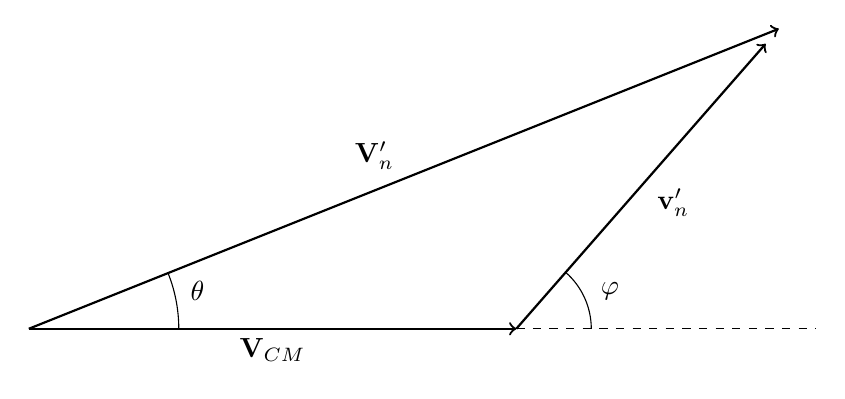
\begin{tikzpicture}[x=0.25in,y=0.25in,scale=0.75]
  \draw [->,thick] (0,0) -- (13,0);
  \draw (6.5,0) node[anchor=north] {$\vec{V}_{CM}$};

  \draw [->,thick] (0,0) -- (20,8);
  \draw (10,4) node[anchor=south east] {$\vec{V}_n'$};

  \draw [->,thick] (13,0) -- (19.65,7.6);
  \draw (16.5,4) node[anchor=north west] {$\vec{v}_n'$};

  \draw [dashed] (13,0) -- (21,0);

  \draw (15,0) arc [start angle=0, end angle=48.84, radius=2];
  \draw (15.5,1) node {$\varphi$};

  \draw (4,0) arc [start angle=0, end angle=21.8, radius=4];
  \draw (4.5,1) node {$\theta$};
\end{tikzpicture}
\caption{Relationship between final neutron velocities in LAB and CM.}
\label{fig::scatteringVelLABvsCM}
\end{figure}

From this diagram, we can apply the law of cosines to find
\begin{equation}
  V_n'^2 = V_{CM}^2 + v_n'^2 + 2 V_{CM}v_n'\cos(\pi-\varphi)
\end{equation}
which simplifies to
\begin{equation}
  V_n'^2 = \left[ \frac{A^2+1}{(A+1)^2} + 2 \frac{A}{(A+1)^2}\cos(\varphi) \right] \vec{V}_n^2.
\end{equation}
An immediate implication of this expression is the relationship between the final and initial kinetic energies of the neutron and the scattering angle in the CM system:
\begin{align}
  \frac{E_n'}{E_n} = \frac{V_n'^2}{\vec{V}_n^2}
                   = \frac{(1+\alpha) + (1-\alpha) \cos(\varphi)}{2}
\end{align}
where
\begin{align}
  \alpha = \left( \frac{A-1}{A+1} \right)^2
\end{align}

To understand this a bit better let's consider a few limiting cases.
\begin{description}
\item[{\(A=1\) :}] This is the case of a neutron scattering off a hydrogen nucleus, and \(\alpha = 0\).  For a glancing collision, the angle of deflect (\(\varphi\) or \(\theta\)) will be very small.  Thus \(E_n' \approx E_n\) and no appreciable energy is lost in the collision.  For a direct hit, in which case the neutron bounces straight back (\(\varphi = \theta = \pi\)) we have \$E\(_{\text{n}}\)' = 0\$--the neutron lost \emph{all} of its energy in a single collision.
\item[{\(A>>1\) :}] In this case the neutron hits something big, and \(\alpha \approx 1\).  Under these circumstances \(E_n' \approx E_n\) \emph{regardless} of the deflection angle.  Think of throwing a tennis ball against a brick wall.
\end{description}

Another important ramification is that for any fixed size of the target nucleus, \(A\), their is a limited range of possible final energies for the neutron.  The largest energy loss will occur when the neutron is scattered directly backward, in which case \(E_n' = \alpha E_n\).  On the other hand, for a small-angle glancing collision, the final energy will be only slightly less than the initial energy and \(E_n' \approx E_n\).  Note that under our current assumptions (namely, that the target nucleus is stationary) the neutron will never \emph{gain} energy.

The preceding work shows us that the amount of energy lost by a neutron depends on the mass of the target nucleus and the cosine of the deflection angle in the CM system.  We can derive a similar relationship between the energy loss and the cosine of the deflection angle in the LAB system, which is often more useful from simulation perspective.

Again starting with the diagram and using the law of cosines we have
\begin{align}
  v_n'^2 = V_n'^2 + V_{CM}^2 - 2 V_n' V_{CM} \cos\theta.
\end{align}
This simplifies to 
\begin{align}
  \left( \frac{A}{A+1} \right)^2 V_n^2 = V_n'^2 + \left( \frac{1}{A+1} \right)^2 V_n^2 - \frac{2}{A+1} V_n' V_n \cos\theta.
\end{align}
Multiplying by the mass of a neutron squared divided by four (to get an expression in terms of energies) and solving for \(\cos\theta\) yields
\begin{align}
  \cos\theta = \frac{1}{2}\left( A+1 \right) \sqrt{\frac{E_n'}{E_n}}
             - \frac{1}{2}\left( A-1 \right) \sqrt{\frac{E_n}{E_n'}}.
\end{align}

\subsection{Reactions Involving a Compound Nucleus}
\label{sec:orgheadline5}
Elastic scattering may be viewed a billiard ball collision.  The neutron and nucleus exchange kinetic energy and linear momentum but nothing else.  In collisions such as inelastic scattering, neutron capture, and fission however, the neutron and nucleus combine to form a new, compound nucleus.  Moreover, this compound nucleus will generally be in an \emph{excited} state, having received additional internal energy from the collision.  We may write such a reaction as
\begin{align}
  \leftidx{^A_Z}{X}{} + \leftidx{^1_0}{n}{} 
  \rightarrow \leftidx{^{A+1}_Z}{X}{^*}
\end{align}
where the * symbol is used to indicate an excited state.  The first reaction in this process is the absorption of a neutron into the target nucleus.  The resultant excited nucleus will then decay, generally on a time scale of \(10^{-14}\) to \(10^{-21}\) seconds.

There are two sources of the excitation energy in a compound nucleus.  First, there is the kinetic energy that is available to the reaction.  This energy, \(e_{\text{exc}}\), is the total pre-collision kinetic energy of the neutron and nucleus in the CM reference frame.  Second, there is a potential source of energy arising from the change in binding energy between the original and compound nuclei.  This change in energy may be expressed as
\begin{align}
  \Delta BE = \left[ M(A,z) + m_n - M(A+1,Z) \right] c^2
\end{align}
where \(M(A,Z)\) is the mass of nucleus \(\leftidx{^A_Z}{X}{}\), \(m_n\) is the mass of the neutron and \(c\) is the speed of light in a vacuum.  Thus the total energy available to the reaction is \(e_{\text{exc}} + \Delta BE\).

Figure \ref{fig::compoundNucleus} shows a cartoon depicting the excitation of a nucleus following neutron capture and three possible de-excitation processes (also called \emph{decay channels}).  Elastic scattering has already been discussed, and as we will see, can be treated as a special case of inelastic scattering, which we will now discuss.
\usetikzlibrary{decorations.pathmorphing}
\begin{figure}
\centering
\begin{tikzpicture}[x=0.25in,y=0.25in,scale=0.75]
  \draw (17,0) node [anchor=north] {$\leftidx{^{A+1}_Z}{X}{}$};
  \draw (14,0) -- (20,0);
  \draw (14,6) -- (20,6);
  \draw (14,11) -- (20,11);
  \draw (14,15) -- (20,15);
  \draw (14,18) -- (20,18);
  \draw (14,20) -- (20,20);
  \draw (14,22) -- (20,22);
  \draw (14,23.5) -- (20,23.5);
  \draw (14,0) -- (14,25);
  \draw (20,0) -- (20,25);

  \draw (7,17) node [anchor=north] {$\leftidx{^A_Z}{X}{}$};
  \draw (4,17) -- (10,17);
  \draw (4,21) -- (10,21);
  \draw (4,24) -- (10,24);
  \draw (4,17) -- (4,25);
  \draw (10,17) -- (10,25);

  \draw [dashed] (14,23.5) -- (0,23.5);
  \draw [dashed] (20,17) -- (0,17);
  \draw [dashed] (14,0) -- (0,0);

  \draw [<->,thick] (2,0) -- (2,17);
  \draw (2,8.5) node [fill=white] {$\Delta BE$};

  \draw [<->,thick] (2,17) -- (2,23.5);
  \draw (2,20.25) node [fill=white] {$e_\text{exc}$};

  \draw [->,thick] (15,23.5) -- (6,21);
  \filldraw [fill=white, draw=black] (12,22.6) circle [radius=0.15in];
  \draw (12,22.6) node {1};

  \draw [->,thick] (16,23.5) -- (8,17);
  \filldraw [fill=white, draw=black] (12,20.25) circle [radius=0.15in];
  \draw (12,20.25) node {2};

  \draw [->,decorate,decoration={snake}] (6,21) -- (6,17);
  \draw [->,decorate,decoration={snake}] (17,23.5) -- (17,15);
  \draw [->,decorate,decoration={snake}] (18,23.5) -- (18,11);
  \draw [->,decorate,decoration={snake}] (19,23.5) -- (19,6);
  \filldraw [fill=white, draw=black] (17.8,10) circle [radius=0.15in];
  \draw (17.8,10) node {3};

  \draw [->] (22,0) -- (22,4);
  \draw (22,2) node [anchor=west] {$E$};
\end{tikzpicture}
\caption{Formation of a compound nucleus following neutron capture.  The decay channels shown are \textcircled{1} inelastic scattering, \textcircled{2} elastic scattering, and \textcircled{3} radiative capture.}
\label{fig::compoundNucleus}
\end{figure}

\subsection{Inelastic Scattering}
\label{sec:orgheadline6}
Inelastic scattering involves the formation of a compound nucleus which subsequently decays through the emission of a neutron and one or more photons (\(\gamma\) rays):
\begin{align}
  \leftidx{^A_Z}{X}{} + \leftidx{^1_0}{n}{} 
  \rightarrow \leftidx{^{A+1}_Z}{X}{^*}
  \rightarrow \leftidx{^A_Z}{X}{} + \leftidx{^1_0}{n}{} + \gamma
\end{align}
The presence of the photon at the end of this reaction clearly indicates that energy has not been conserved between the neutron-nucleus pair.  What has happened instead, is that upon ejection of the neutron, the \(\leftidx{^A_Z}{X}{}\) was actually left in an excited state and emitted one (or more) photons to return to the ground state.

When considering the energetics of inelastic scattering, note that the final nucleus is simply the original target nucleus.  Thus the role of the change in binding energy has no net effect on the energy of the system.  There was \(e_\text{exc}\) energy available before the collision (from the kinetic energy of the neutron and nucleus) and there is still \(e_\text{exc}\) energy available after the collision, although the photon has appeared and claimed part of the available energy.

A second consideration is that for the compound nucleus to decay into an excited state, there must have been at least enough energy, \(e_\text{exc}\), to bridge the gap between the ground and the first excited state of the original nucleus.  Otherwise there would not have been enough energy available after the neutron emission for the target nucleus to be in an excited state!  This type of reaction is known as a \emph{threshold} reaction, because the energy of the colliding pair must meet a certain "threshold" value before the reaction can take place.  Note that if the compound nucleus emits a neutron and returns the target nucleus to its ground state, then there is no photon emission (which is only a result of de-excitation), thus the total energy of the reaction \(e_\text{exc}\) is shared between the neutron and nucleus as kinetic energy.  This, however, implies overall conservation of kinetic energy between the neutron and nucleus, thus it is an \emph{elastic} scattering event!

\subsection{Radiative Capture}
\label{sec:orgheadline7}
A radiative capture reaction is essentially an inelastic neutron scattering \emph{without the neutron}.  That is, the target nucleus absorbs a neutron then de-excites simply by emitting one or more photons:
\begin{align}
  \leftidx{^A_Z}{X}{} + \leftidx{^1_0}{n}{} 
  \rightarrow \leftidx{^{A+1}_Z}{X}{^*} + \gamma
\end{align}
Note that the total amount of energy to be relieved through the emission of photons is \(e_{\text{exc}} + \Delta BE\).

\subsection{Fission Reactions}
\label{sec:orgheadline8}
In a fission reaction, the energy \(e_{\text{exc}} + \Delta BE\) is enough to overcome the fission barrier (which is an energy threshold), and the nucleus splits into two fragments plus several free neutrons and photons.  The nuclear configuration of the fission fragments and the number of free neutrons emitted are both statistical quantities.  
\section{References}
\label{sec:orgheadline10}
\begin{itemize}
\item \href{Hebert2009}{Hebert}
\item \href{Duderstadt:Hamilton1976}{Duderstadt and Hamilton}
\item \href{Stacey2001}{Stacey}
\end{itemize}
\end{document}